% !TEX root = ./thesis.tex

\chapter{Model}

In this chapter we provide overview of our method.
First we provide details about our model initialization and training procedure.
Than we describe baseline architectures that we used as the backbone of our model during evaluation.
At last, we describe our method of robust manifold learning.


\label{ch:mode}

\section{Training process}

In our training we use a server with Intel Xeon CPU 2.40GHz, 64GB of RAM and a GeForce GTX TITAN X Kepler graphics card with 12GB of video memory. Server runs Debian 8.7 operation system with CUDA 8.0, CuDNN 5.1 and TensorFlow 1.0 installed.

\subsection{Tensorflow}

In deep learning TensorFlow \cite{GoogleResearch2015, Abadi2016}, Torch \cite{torch}, and Caffe \cite{jia2014caffe} are among the most common choices of scientific computing framework.
These frameworks use different underlying programming languages and show different compatibility features and qualities of managing computational resources.

We use TensorFlow as our scientific computing framework of choice.

TensorFlow is an open source cross platform software library.
TensorFlow constructs complex computational procedures in form of computational graphs.
Nodes of the computational graph represent some mathematical operations.
Edges of the graph represent data flow between nodes in form of multidimensional arrays, also called tensors.

\begin{figure}[h!]
  \centering
    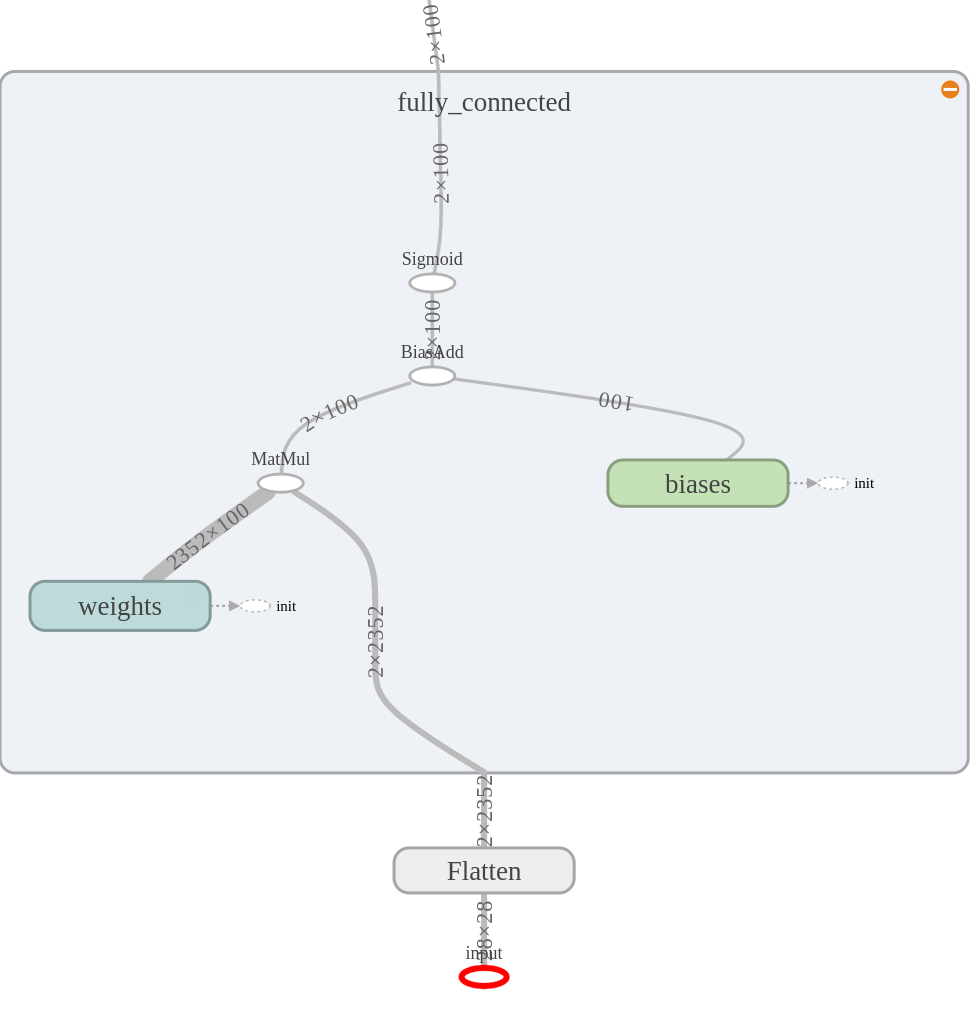
\includegraphics[width=0.7\textwidth,height=0.7\textheight,keepaspectratio]{tf_graph_1.png}
  \caption{TensorFlow detailed graph representation of a single fully connected layer with 100 neurons and sigmoid activation function. Image produced with the build in visualization tool.}
  \label{fig:tf_graph}
\end{figure}

TensorFlow provides cross platform compatibility, which allows to run code on different types of devices and operation systems.
Abstraction over underlying system allows to run models, build with TensorFlow, both on GPUs and CPU without code changes.
Integration with hight performance computing libraries as CUDA \cite{Nickolls2008} and native support of distributed computing makes it a good candidate for computer vision tasks.
An competition winning family of convolutional neural networks Inception is solely developed and maintained on that platform \cite{Szegedy2016}.

We use TensorFlow as our framework of choice for several reasons.
First of all, being a crossplatform frameworks it enables larger audience to reuse results of our research.
Second, it allows to easily configure and run deep network architecture and, at the same time, apply non-trivial modification to the computational flow.
And, at last, it provides build-in visualization tools that allow better control of the learning process.

All our code is shared for public use under MIT License.
\footnote{\url{https://github.com/yselivonchyk/TensorFlow_DCIGN}}

\subsection{Training algorithm}

We run the training using stochastic gradient descent algorihtm with mini-batches \ref{alg:bp}. We use adaptive learning rate in form of Adam update rule \ref{alg:adam}. Adaptive learning rate rule has shown to lead to convergence of the backpropagation algorithm at least as often as other methods. It also showed to converge consistently even for a single learning rate for different models.

We use mini-batch size of 128 as the largest one that fits into video memory for each model.
We also found that gradient descent convergence for each of the tested models with learning rate $\nu=0.0001$ is used. This learning rate falls into the interval of recommended learning rates for Adam update rule \cite{Kingma2015}.

We use early stopping as the termination condition of the algorithm \ref{alg:bp}.

To select hyper-parameters of the model, such as weights $\alpha, \beta$ of a composite error $L=L_1 + \alpha L_2 + \beta L_3$, layer sizes etc. we perform a single grid search per parameter.
Grid search is executed for a single parameter at a time, while other parameters stay fixed.
In each grid search is performed for 3 values $\{p_1, p_2, p_3\}$. Whenever better results are achieved for border values $p_1$ or $p_3$, the grid is shifted in the direction of the winning value. When middle value $p_2$ shows the best result but the difference is significant grid search is repeated for decreased grid size.
When parameter shows no effect on model performance the value, that causes better computational efficiency of the model, is selected.

\subsection{Model parameter initialization}

Initial model parameters $\theta$ in conjunction with learning algorithm play crucial role in finding good local minima of optimization problem.
Gradient descent algorithm does not guarantee convergence in finite number of steps.
Hence, model parameters can stay in a "noisy" region where, regardless of learning rate, step in the direction of the gradient on average causes zero decrease of the loss.

It has been shown, that bad weight initialization can lead to exploding or dying out signal especially in deep architectures \cite{Glorot2010}. More specifically, for very small initial weights signal propagating to the further layers becomes too small to be useful and vise versa.
Too large and too small pre-activation values can lead to saturation of sigmoid or tangent units and to dying out of ReLU units. This effectively decreases number of learning units in the network and can impede training.

Most commonly, \textit{Xavier initialization} is used with deep neural networks to avoid situation as described above \cite{Glorot2010}.
Another options might include layer-wise weight initialization, pre-training of the parts of the model \cite{Simonyan2015} or applying weight regularization \cite{Good2016}.
Yet, we would prefer the issue of weight initialization not to effect the training process.


Xavier initializer suggest using normalized initialization, that depends on the number of inputs and ouputs of the layer \cite{Good2016}. Weight values are drown uniformly at random from a normal distribution $\Bbb{U}$:

\begin{equation}\label{eq:xavier}
  w_{j, i} \sim \Bbb{U}(
  \mu=-\frac{\sqrt{6}}{\sqrt{n_j+n_{j+1}}},
  \sigma=\frac{\sqrt{6}}{\sqrt{n_j+n_{j+1}}})
\end{equation}

where $i\in\{0, \ldots, |W_j|\}$ is a index of a weight in layer $j$ and $n_j$ is a number of input units of the layer $j$.


\section{Backbone architectures}

In this section we provide overview of three network architectures that we consider useful for trajectory learning from visual data.

All architectures follow multilayer autoencoder design.
Regardless of the backbone, design the last layer of the encoder is a fully connected layer with small (typically smaller than 4) number of computational units.
We would refer to the outputs of this layer as to  \textit{input encoding}.
Additional constrains applied to the encoding are described in section \ref{ss:mf}.

Throughout this work we stick to \textit{mirrored} designed of the encoder and decoder.
This approach allows to have balanced complexity of encoder and decoder subnetworks.

Learning objective of an autoencoder is to reconstruct the original image.
We use $L_2$ $norm$ as the reconstruction loss $L_{reco}$:

\begin{equation}
  L_{2} = \frac{1}{2} \sum_{i, j, c} (x_{i,j,c} - \hat{x}_{i,j,c})^2
\end{equation}

where $x, \hat{x}$ are original image and network output correspondigly.

Input images are encoded in RGBD format. It means that each image pixel $x_{i,j} \in \Bbb{U}^4$ is a 4-dimensional vector.
Each color channel of pixel vector $x_{i,j}$ is a discrete value between 0 and 255: $\Bbb{U} = \{0, 1, \ldots, 255 \}$.
We follow a common practice and treat values discrete values of set $\Bbb{U}$ as continuous values in range $[0.0, 255.0]$.

We scale down input values to allow potential perfect reconstruction by the network.
Scaling is necessary, since activation functions as logistics sigmoid or hyperbolic tangent are upper bounded by 1.0.


\subsection{Fully connected autoencoder}

Fully connected layer of neural networks is a set of computational units, each of which relies on the full set of input parameters of the layer and produces a single output.
We use computational units as described by \ref{eq:per}. We use logistics sigmoid as an activation function.
In this form each fully connected layers with $n_{i-1}$ inputs and $n_i$ outputs rely on $|W_i|=n_{i-1}*(n_i+1)$ parameters.

Work by Jaderberg et al. \cite{Jaderberg2015} suggests, that a fully connected neural network with a single hidden layer might be sufficient to capture spacial information about the input.
In this work, a fully connected \textit{localization net} with a single hidden layer and small number of output units (up to 6) is used to produce transformation parameters for visual data input.
We believe that this architecture represents the most trivial design and use it as a reference backbone model.

Another group of authors successfully applied fully-connected autoencoder to learn latent input representation using Generative Moment-Matching networks \cite{Li2015}. In their experiment, fully connected autoencoders were able to construct dense manifold of the input. For small datasets as MNIST and Toronto Faces Dataset \cite{tfd,lecun-mnisthandwrittendigit-2010} 2 or 3 layers in encoder and decoder networks were sufficient.

Fully connected layers rely on huge number of parameters comparing to convolutional and deconvolutional layers.
Number of parameters grows fast with increase in number of layers or number of output units.
This growth of complexity of parameter space can lead to over-fitting in form of identity learning by the network.

A typical design of an autoencoder network is described by table ?? and depicted on figure ??.

\subsection{Convolutional autoencoder}

Convolutional models are showing best results in various computer vision competitions in the recent years \cite{ILSVRC15, Zhou2016}.

Convolutional layers of neural networks rely on relatively small number of parameters.
Convolutional neurons typically share the parameters across a single feature map \ref{eq:conv}.

ReLU \cite{Nair2010}

\begin{figure}[h!]
  \centering
    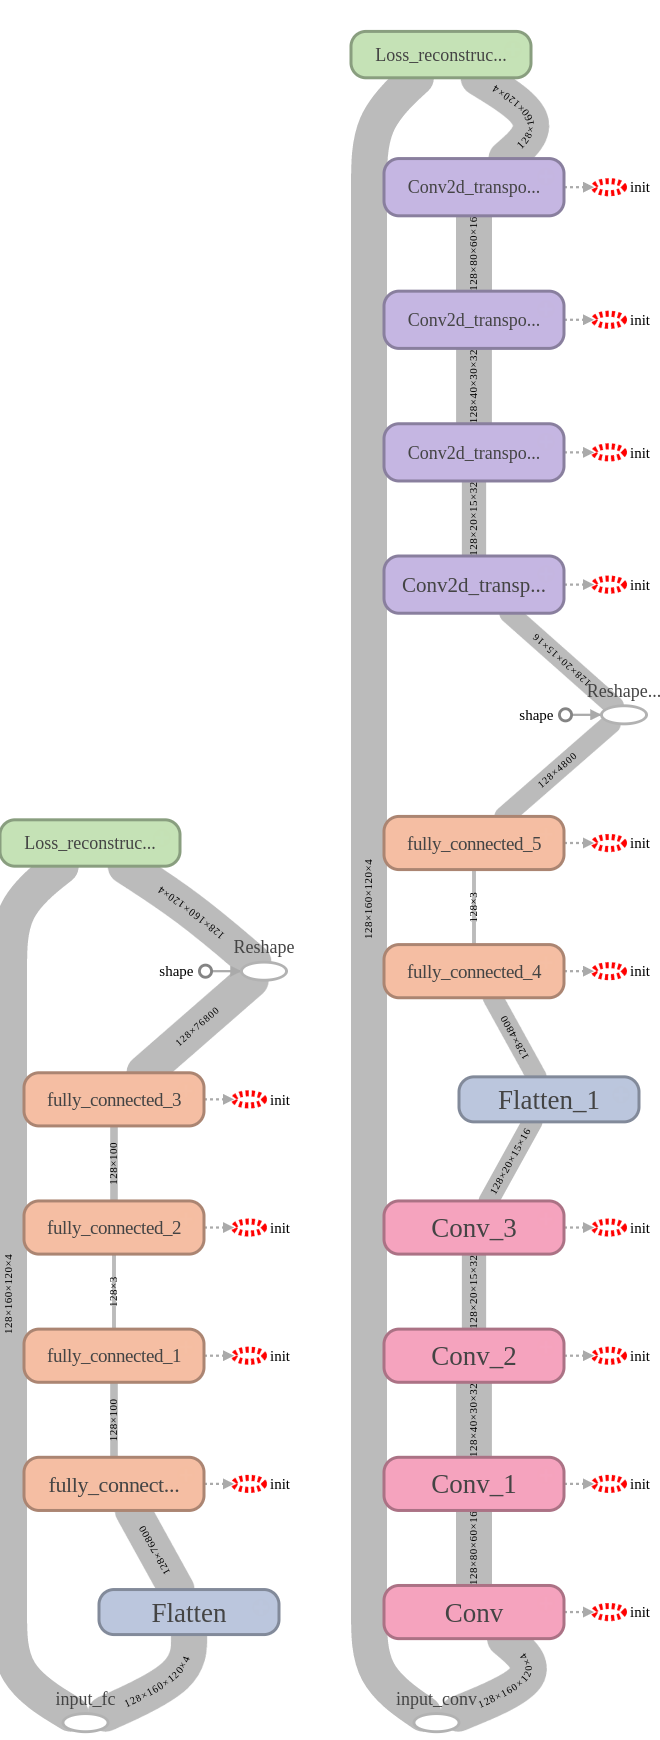
\includegraphics[width=\textwidth,height=\textheight,keepaspectratio]{backbone_1.png}
  \caption{TensorFlow detailed graph representation of a single fully .}
  \label{fig:tf_graph}
\end{figure}

\subsection{WhatWhere autoencoder}

Architecture of What-Where autoencoders \cite{Zhao2015} propose using additional information flow between encode and decoder to improve quality of reconstruction.
What-where autoencoders store the positions of maximum-elements during max-pooling operation to reuse it during reconstruction.
Given positional information decoder no longer have to "guess" the relative position of pooled features during upsampling.

What-where autoencoders in the encoder part use the same architecture as convolutional counterpart.
In the decoder part of the network in addition to transposed convolution \ref{ch:tcnn} an updated upsampling operation is used. Updated upsampling operation called \textit{unpooling} is described in section \ref{ch:unp}.

We consider What-Where autoencoders to be useful for interpretable feature learning, since positional information flow should simplify the process of learning good image reconstruction. This simplification can possibly lead of lesser impact of the noisy $L_{reco}$ error on the learning process.

\begin{figure}[h!]
  \centering
    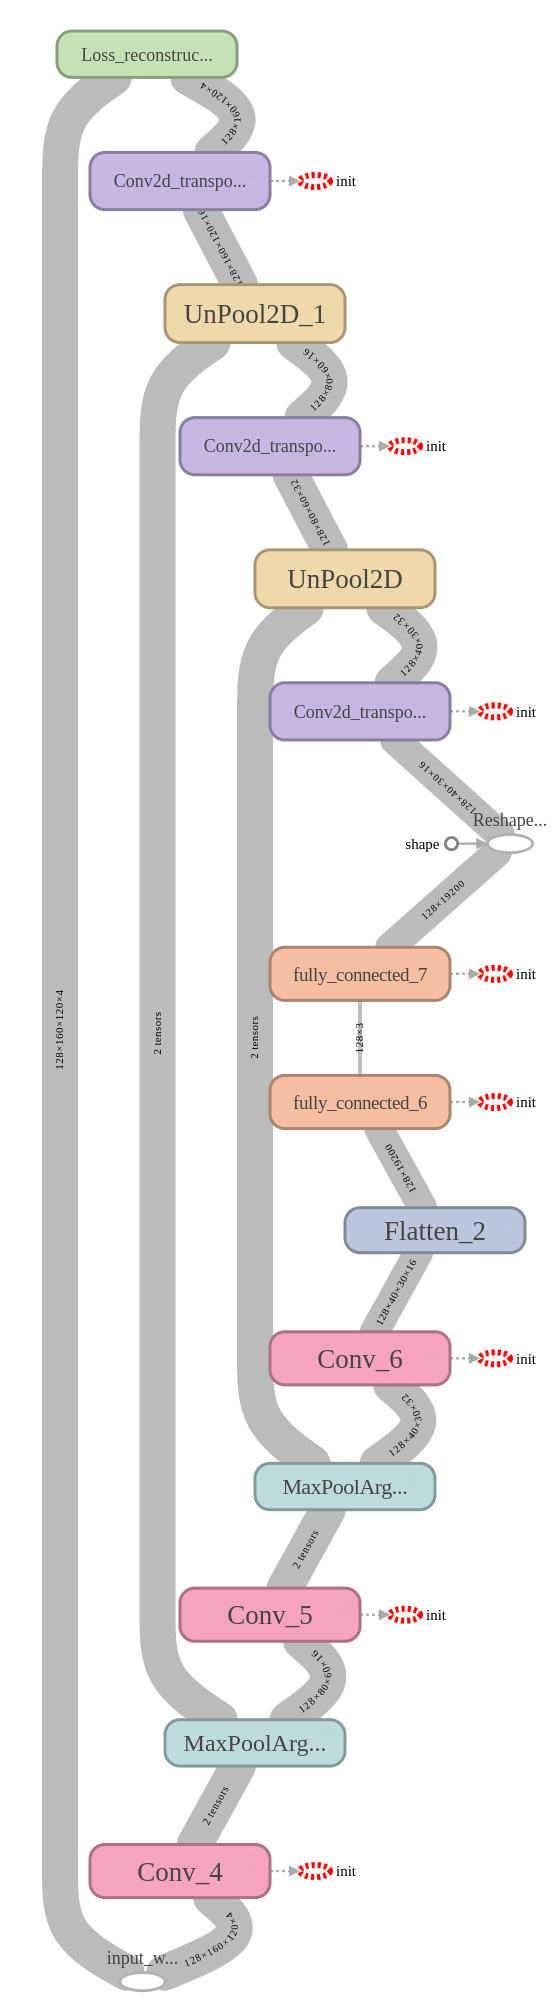
\includegraphics[width=\textwidth,height=\textheight,keepaspectratio]{backbone_2.png}
  \caption{TensorFlow detailed graph representation of a single.}
  \label{fig:tf_graph}
\end{figure}

\section{Model pretraining}



\section{Manifold learning}\label{ss:mf}
\subsection{Predictive objective}
\subsection{Denoising regularization}
\subsection{Feature set regularization}
